% ============================================================================
\chapter{Data and Methodology}\label{ch:data}
% ============================================================================

% ============================================================================
\section{Data}\label{sec:data}
% ============================================================================

All experiments use end-of-day SPX option quotes from OptionMetrics IvyDB US, accessed through
WRDS under secid \texttt{108105}. The sample runs from 2 January 2018 to 29 August 2025 and
contains 1,926 trading days. It covers several distinct market regimes, including Volmageddon,
the COVID-19 crash, the 2022 monetary tightening cycle, and the 2024 to 2025 period.

Five OptionMetrics tables enter the pipeline: the option-quote table, the zero-coupon yield
curve, the forward-price table, the proprietary volatility surface, and a historical-volatility
series. The proprietary surface is used only as an industry benchmark and never as training
input. The CBOE \texttt{VIX\_History} file provides the published VIX series used for the
external validation in Section~\ref{sec:vix}.

Notebook~NB01 transforms the raw tables into a single reproducible Parquet dataset used by all
subsequent notebooks. Each cleaning rule is stated explicitly and enforced by an automated test
before the dataset is written to disk.

\subsection{Coordinates and feature engineering}\label{sec:coords}

For each quote, we define the maturity $\tau=\frac{\mathrm{DTE}}{365}$ using the ACT/365 convention. We also compute the mid price and quoted half-spread as
\[
\mathrm{mid}=\frac{\mathrm{bid}+\mathrm{ask}}{2},
\qquad
\mathrm{halfspread}=\frac{\mathrm{ask}-\mathrm{bid}}{2}.
\]
Log-moneyness is defined by $k=\log\!\left(\frac{K}{F}\right),$
where $F$ denotes the forward associated with the quote's expiry. Strikes are rescaled from the OptionMetrics convention using $K=\frac{\texttt{strike\_price}}{1000}.$

A quote is classified as \emph{out of the money} when $k\ge0$ for a call or $k<0$ for a put.
Only the OTM side is retained because it is generally the more liquid and informative side of
the volatility smile. It is also the object reconstructed by every model in this thesis.

\subsection{Cleaning rules}\label{sec:cleaning}

Cleaning is implemented as a lazy query plan so that filters reduce the data before
materialisation.

\paragraph{Quality filters.}
A quote is retained only if its bid is strictly positive and its market is not crossed: $0<\mathrm{bid}\le\mathrm{ask}.$
Maturity must lie between $7$ and $730$ calendar days. Shorter maturities are strongly affected
by microstructure noise, while longer maturities are comparatively illiquid. The call and put
indicator must belong to $\{\mathrm{C},\mathrm{P}\}$.

\paragraph{Missing implied volatility.}
Approximately $5.7\%$ of the raw rows have no reported implied volatility. Delta and vega are
also missing on exactly these rows, so the Greeks cannot be used to recover the volatility.
About $99.98\%$ of the affected observations are deep in-the-money options. Their prices are
almost entirely intrinsic value, which makes a reliable Black inversion difficult relative to
the quoted spread.

Only about $118$ of the $8.5$ million rows with missing implied volatility are OTM. Since the
thesis reconstructs the OTM surface and this residual count is negligible, all rows with
missing implied volatility are removed rather than repaired.

\subsection{Forwards and discount factors}\label{sec:forwards}

The quote-level forward is retained whenever it is available. Missing values are filled from
the OptionMetrics forward table through a left join on $(\texttt{secid},\texttt{date},\texttt{expiry},\texttt{settlement}).$
Every retained quote therefore has a valid forward for the construction of the log-moneyness.

The zero-curve rate at the nearest available horizon is then attached through an as-of join for
each trading date. The corresponding discount factor is $D=e^{-r\tau}.$

\begin{figure}[!htbp]
    \centering
    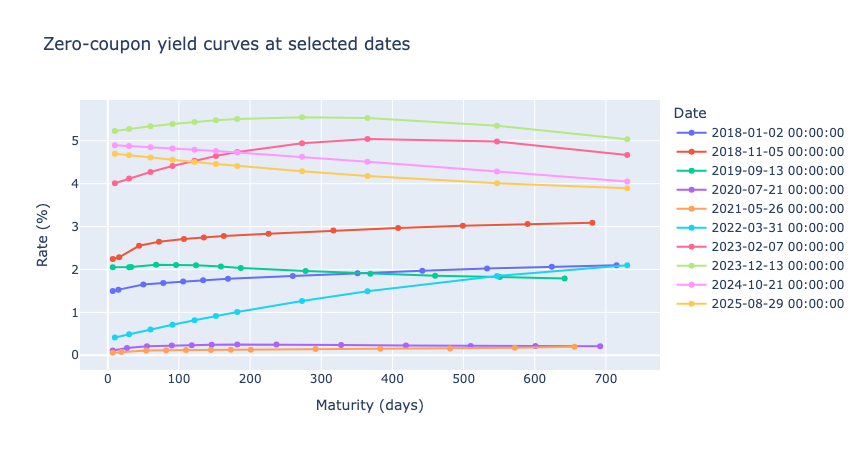
\includegraphics[
        width=0.92\linewidth,
        trim=0 0 0 2.5cm,
        clip
    ]{figures/nb01_c08_0.png}
    \caption{OptionMetrics zero-coupon yield curves on selected trading dates. The curves are
    used to construct the discount factors required for quote validation.}
    \label{fig:nb01curves}
\end{figure}

\subsection{One expiry, one contract}\label{sec:collision}

Standard SPX options are generally AM-settled, while SPXW weekly options are PM-settled. The two
families can share an expiration date while trading at slightly different prices. Retaining
both would create two implied volatilities for the same approximate $(k,\tau)$ location.

Each collision is therefore resolved deterministically in favour of the AM-settled SPX
contract. A diagnostic verifies that no pair
$(\texttt{date},\texttt{expiry})$ retains more than one contract type.

Contract identity is preserved throughout the procedure. Expiries are not merged by rounded
values of $\tau$ because this produces artificial sawtooth patterns in the term structure.

\subsection{Independent implied-volatility validation}\label{sec:ivcheck}

The transformation from raw quotes to $(k,\tau,w)$ depends on the forward, discount factor,
coordinate change, and implied-volatility inversion. A silent error in any of these components
would contaminate the complete dataset.

We therefore recompute implied volatility independently for every eligible quote using
vectorised bisection on the Black--76 price. The result is compared with the OptionMetrics value
$\mathrm{iv}_{\mathrm{OM}}$. Inversion is attempted only when the observed price satisfies the
relevant no-arbitrage bounds. This provides an initial quote-level arbitrage screen.

A small median difference between the recomputed volatility and
$\mathrm{iv}_{\mathrm{OM}}$ validates the forward, discount, coordinate, and inversion code
jointly.

\subsection{Reproducibility guardrails}\label{sec:guardrails}

All diagnostics are converted into blocking tests before the clean Parquet file is written.
The notebook stops rather than producing a dataset when any required assumption fails. The
tests verify that only the expected SPX secid remains, that every maturity satisfies the DTE
filter, and that every bid is positive. They also exclude crossed markets and require complete,
finite values of $k$ and the OTM indicator. Finally, they verify that no expiry retains multiple
contract types.

Once all tests pass, the clean dataset is written to disk. Figure~\ref{fig:nb01counts} reports
the number of retained OTM quotes through time. Figure~\ref{fig:nb01cloud} illustrates the
sparse and irregular geometry of the resulting input on a representative trading day.

\begin{figure}[!htbp]
    \centering
    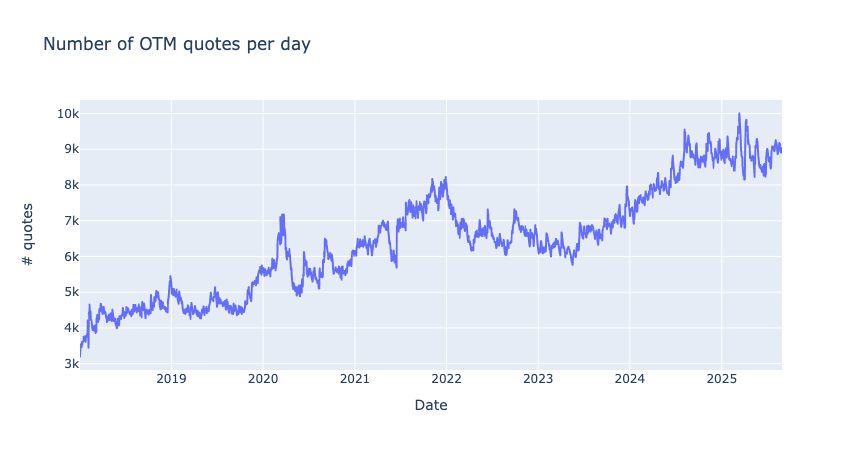
\includegraphics[
        width=0.92\linewidth,
        trim=0 0 0 2.5cm,
        clip
    ]{figures/nb01_c24_1.png}
    \caption{Number of OTM quotes retained on each trading day after application of the NB01
    cleaning pipeline.}
    \label{fig:nb01counts}
\end{figure}

\begin{figure}[!htbp]
    \centering
    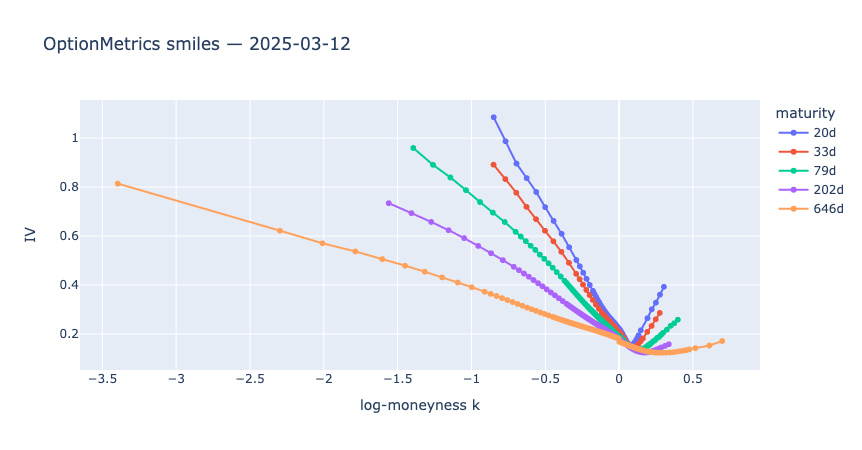
\includegraphics[
        width=0.92\linewidth,
        trim=0 0 0 2.5cm,
        clip
    ]{figures/nb01_c25_0.png}
    \caption{Cleaned OptionMetrics smile cross-section for one trading day across all retained
    expiries. The observations form the sparse, irregular, and noisy input consumed by the
    reconstruction methods.}
    \label{fig:nb01cloud}
\end{figure}

% ============================================================================
\section{Evaluation domains and unified protocol}\label{sec:protocol}
% ============================================================================

Two evaluation domains are used throughout the thesis. The \emph{full quoted domain} retains
the complete observed range and therefore includes deep OTM puts with log-moneyness close to
$k=-2.2$. The \emph{paper domain} is restricted to
$k\in[-0.6,0.4]$, $\mathrm{DTE}\ge10.$
This second domain facilitates comparison with the existing literature.

For each trading day, $20\%$ of the observations are held out separately within each expiry
slice. 
Every model family is consequently evaluated on the same held-out quotes. Content-based seeding
also ensures that staging and production runs remain comparable on a day-by-day basis.

Arbitrage is audited both on the quoted domain and on a capped extension. The extended range is
twice the observed $k$-range and is clipped to $|k|\le1.5.$
This restriction prevents economically irrelevant strikes from inflating the measured
violation rates. For example, auditing at $k=-4.4$ would correspond to a strike near one percent
of spot.

The audit follows conditions (A1) to (A4) of Section~\ref{sec:softtheory}. It uses independent
grids, blind-spot flags, and separate strict and material statistics with $\mathrm{tol}_{\mathrm{mat}}=10^{-3}.$
Stress and invariance conclusions are reported only when their validity gates pass.

Aggregate arbitrage statistics are also conditioned on fit validity through the
\texttt{gated\_*} columns and \texttt{n\_fit\_ok}. A day on which a model fails to fit is
excluded from its arbitrage comparison. Otherwise, numerical non-convergence could be
misreported as an economically meaningful arbitrage violation.

\subsection{Data splits}\label{sec:splits}

Two distinct splitting schemes are used, because the two model families answer different
questions. Both are stated here rather than in the results chapters.

\paragraph{Per-day models.} The parametric benchmark of Section~\ref{sec:parametric} and the
deep smoother of Section~\ref{sec:deep} are fitted independently on each trading day, so there
is no temporal split to make: generalisation is measured \emph{within} the day. On every day,
$20\%$ of the quotes are held out per expiry slice under a deterministic seed
$\mathrm{crc32}(\text{date})$, and the remaining $80\%$ are used for fitting. Because the seed
depends only on the date, every model family in this thesis is scored on exactly the same
held-out quotes, and staging and production runs remain comparable day by day.

\paragraph{Operators.} An operator is trained once across many days, so the split must be
temporal, and it is \emph{chronological} rather than random: the $1{,}926$ trading days are
divided in order into $1{,}155$ training days, $385$ validation days and $386$ test days. The
test set is therefore the final year and a half of the sample, and no training day post-dates a
test day. Every operator number reported in Section~\ref{sec:operator} is consequently a
temporal generalisation claim rather than an in-sample one. The per-day $20\%$ hold-out is
applied \emph{in addition}, so that quote-level and day-level generalisation are measured
separately. Validation days are used only for monitoring and for the choice of training length;
no architecture or hyperparameter is selected on the test set.

\paragraph{Synthetic data.} The synthetic bank used for pretraining is generated independently
of the real sample and never enters validation or test. Its role is to answer a transfer
question, whether certified synthetic surfaces can substitute for data scale in the
academic-data regime, and it is reported as such.

\subsection{Compute infrastructure and execution}\label{sec:compute}

The production runs are too long for a laptop and are executed on a shared multi-core Linux
compute server at T\'el\'ecom Paris, accessed over SSH through the institutional gateway. The
environment is a dedicated conda environment with a CPU build of PyTorch; no GPU is used
anywhere in this thesis, which is worth recording because it constrains the operator training
budgets discussed in Section~\ref{sec:operator}.

\paragraph{Parallelisation by year.} The dominant cost is the per-day deep smoother of
Section~\ref{sec:deep}, which fits one network per trading day and is therefore embarrassingly
parallel across days. The 2018--2025 sample is sharded by calendar year into eight independent
jobs, one per year, executed concurrently on eight cores, with a ninth process handling the
synthetic experiments. Each shard writes to its own output namespace, so no two processes
contend for the same file, and shards can be re-run individually after a failure without
repeating the others. This reduces a sequential run of roughly thirty hours to a wall-clock time
of a few hours.

\paragraph{Detached execution and reproducibility.} Notebooks are executed non-interactively
with \texttt{nbconvert}, so the executed notebook including all outputs is preserved as an
artefact alongside the Parquet files. The whole pipeline is launched inside a \texttt{tmux}
session, which detaches the computation from the SSH connection: the run survives disconnection,
and progress is monitored by tailing per-shard log files. Results are transferred back with
\texttt{rsync}. The practical consequence for reproducibility is that every reported number is
traceable to an executed notebook and a log file, both retained, rather than to an interactive
session that no longer exists.

